% =====================================================================
% VERSION ENSAE, REDUCTION SFE (phase 3, 1er octobre 2026) : chapitre 6, modelisation multi-etats de la conformite.
% Copie a texte constant de chapitres/11_conformite_multietats.tex.
% Ne changent que les titres et les renvois repares, listes dans
% reduction/phase3.md.
% Lu par main_ensae.tex seul : ne jamais le faire lire par main_institut.tex,
% qui garde chapitres/.
% =====================================================================

\chapter{Modélisation multi-états de la conformité}
\label{chap:multietats}


\section{Deux échelles de temps}
% HARNAIS-HORS-SECTION: le seul nombre lu est l'indice de $v_0$ (distribution initiale) dans la legende, une notation et non un resultat.

Que change le passage d'un état non conforme (NC) à partiellement conforme (PC), puis conforme
(C) ? Chaque état fixe les valeurs des quatre canaux du calcul annuel : les incidents et leurs
pertes sont simulés sous ces paramètres. Les états sont supposés, sans observation par entité.

La variable latente ci-dessous décrit une distribution possible des états. Une chaîne de Markov
traite ensuite une question distincte : leur évolution au cours de la remédiation, sur plusieurs
années. Le temps d'une transmission entre piliers et celui d'une amélioration de conformité
restent donc séparés. Cette distinction rejoint les migrations de rating en crédit
(\S\ref{sec:couplage}) et la séparation des échelles de propagation et de calendrier
de \citet{ccrn2026}.

Nous notons $B_e$ le besoin de capital annuel calculé sous un état fixé $e$.
La figure~\ref{fig:deux-horloges} montre comment les probabilités d'état au cours du temps
pondèrent ces capitaux. La trajectoire obtenue est une moyenne de quantiles ; calculer
le quantile d'une perte annuelle dont l'état est lui-même aléatoire demanderait d'agréger
les distributions de pertes avant de prendre le quantile.

\begin{figure}[H]\centering
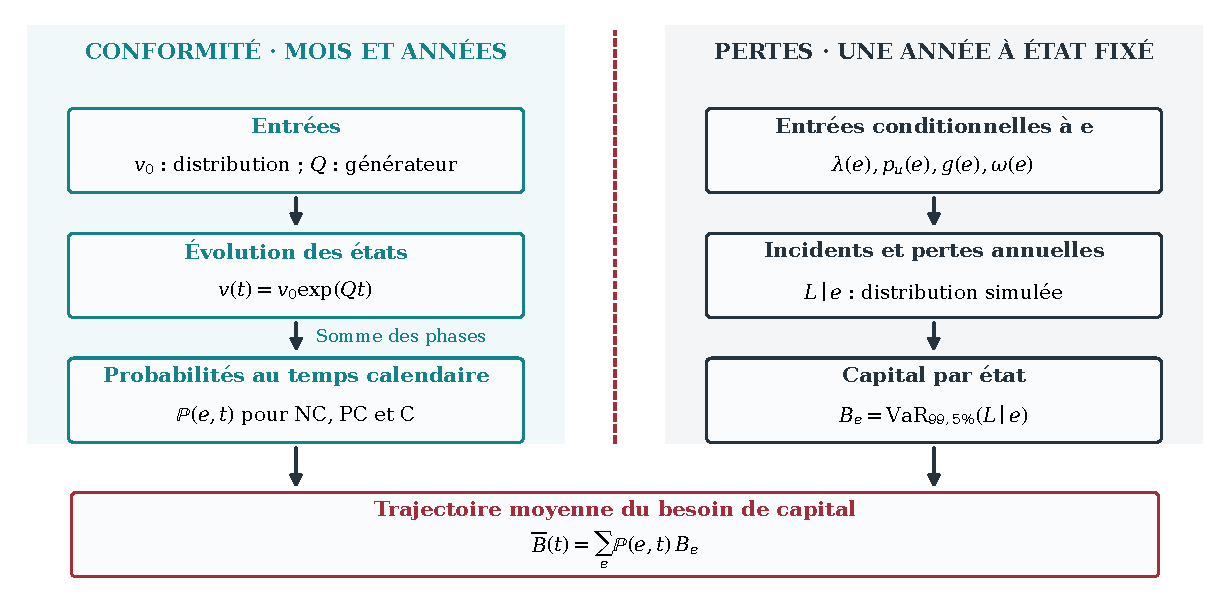
\includegraphics[width=\textwidth]{figures_pedagogie/deux_horloges_conformite.pdf}
\caption{Deux échelles de temps et deux calculs. À gauche, $v_0$ et le générateur de phases $Q$ donnent les probabilités d'état au temps $t$. À droite, chaque état fixe un calcul de pertes sur un an. Leur combinaison donne la moyenne des besoins conditionnels ; elle ne donne pas le quantile des pertes mélangées.}
\label{fig:deux-horloges}
\end{figure}

\section{Vasicek multi-états à seuils ordonnés}

Chaque pilier possède une capacité de conformité latente $C^\star\sim\mathcal N(0,1)$, que nous
décomposons à la Vasicek en un facteur systémique commun $\Theta$ et un choc idiosyncratique $\varepsilon$ propre au pilier. Ce sont deux variables normales centrées réduites et indépendantes, supposées par le modèle et non mesurées ; $\gamma$ est la charge du facteur commun :
\begin{equation}
C^\star \;=\; \gamma\,\Theta \;+\; \sqrt{1-\gamma^2}\,\varepsilon, \qquad \gamma=0{,}68.
\end{equation}
Au lieu d'un unique seuil de défaut, nous en posons deux, ordonnés, qui découpent trois
états :
\begin{equation}
\text{NC si } C^\star\le K_{\text{bas}}, \quad
\text{PC si } K_{\text{bas}}<C^\star\le K_{\text{haut}}, \quad
\text{C si } C^\star>K_{\text{haut}}.
\end{equation}
Les seuils sont fixés par les probabilités d'état ancrées sur les enquêtes de
conformité de fin 2025 ($0{,}35$, $0{,}35$ et $0{,}30$ pour NC, PC et C, annexe~B), d'où $K_{\text{bas}}=\Phi^{-1}(p_{\text{NC}})$ et
$K_{\text{haut}}=\Phi^{-1}(p_{\text{NC}}+p_{\text{PC}})$. Sur le score $U=\Phi(C^\star)$, uniforme sur $[0,1]$, ces seuils sont les coupures $0{,}35$ et $0{,}70$. Ce probit ordonné généralise la latente
de défaut binaire en une latente de conformité à trois niveaux. Sachant l'environnement $\Theta$, on
obtient
\begin{equation}
\mathbb P(\text{NC}\mid\Theta)=\Phi\!\Big(\tfrac{K_{\text{bas}}-\gamma\Theta}{\sqrt{1-\gamma^2}}\Big),
\qquad
\mathbb P(\text{C}\mid\Theta)=1-\Phi\!\Big(\tfrac{K_{\text{haut}}-\gamma\Theta}{\sqrt{1-\gamma^2}}\Big).
\end{equation}
Intégrée sur $\Theta$, la marginale redonne l'ancrage, tandis qu'en crise systémique la masse bascule
vers la non-conformité (figure~\ref{fig:multietats-rapport}).

\begin{figure}[H]\centering
\figover{S10_scr_multi_etats.png}
\caption{États de conformité et capital. (A)~Besoin de capital du périmètre financier étudié par état, en cumulant la fréquence seule,
puis la propagation, puis la détection, trois des canaux définis au
\S\ref{sec:quatre-canaux}. (B)~Probabilités d'état en régime normal et en crise systémique : la
masse bascule vers la non-conformité.}
% SOURCES-SCRIPTS: 16
\label{fig:multietats-rapport}
\end{figure}

% SOURCES-SCRIPTS: 63


\section{Quatre canaux de la conformité}
\label{sec:quatre-canaux}

Nous comparons les états en modifiant quatre entrées du même calcul annuel.
La figure~\ref{fig:deux-etats-calcul} donne leurs valeurs aux deux extrêmes, lorsque tous les
piliers partagent le même état (\S\ref{sec:etat-par-pilier}). Les lois de perte de base et
l'agrégation sont conservées ; les différences entre les entrées restent des scénarios.

\begin{figure}[H]\centering
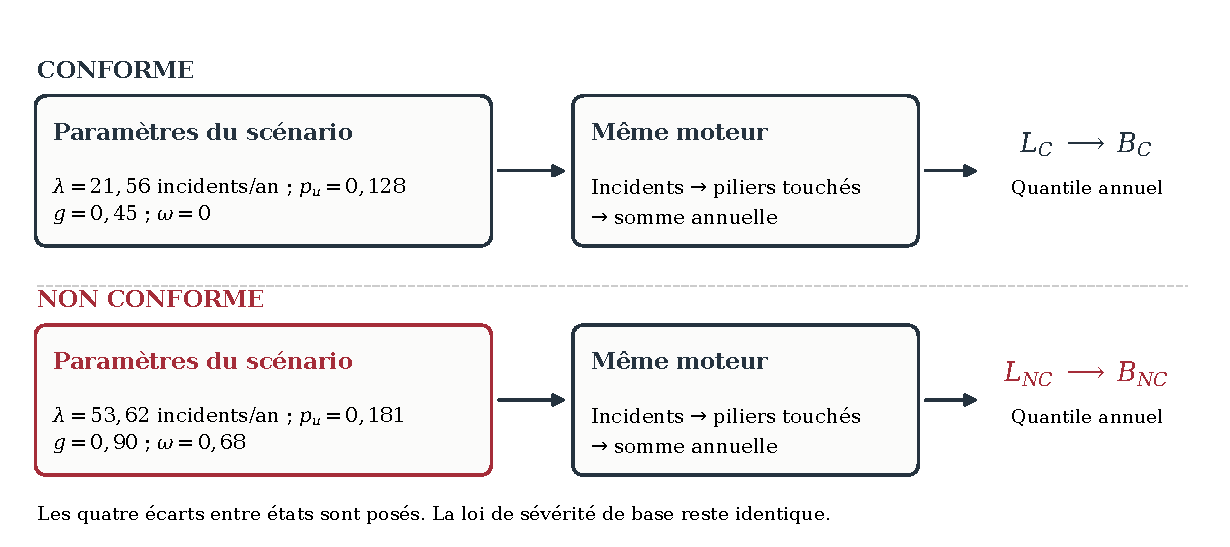
\includegraphics[width=\textwidth]{figures_pedagogie/deux_etats_meme_calcul.pdf}
\caption{Deux états supposés, un même calcul annuel. $\lambda$ règle le nombre d'incidents, $p_u$ le dépassement par pilier, $g$ la propagation et $\omega$ le choc commun. $L$ désigne la perte annuelle et $B$ son quantile à $99{,}5\,\%$.}
\label{fig:deux-etats-calcul}
\end{figure}

\begin{enumerate}[leftmargin=1.5em,itemsep=2pt,topsep=2pt]
\item L'état module la \emph{fréquence} $\lambda$ des incidents amorcés par un multiplicateur de
  scénario, de $21{,}56$ incidents enregistrés par an à l'état conforme à $53{,}62$ à l'état non
  conforme.
\item Le gain de \emph{propagation} $g$ de la normalisation~\eqref{eq:norm} baisse de $0{,}90$ à
  $0{,}45$, car une entité plus conforme contient mieux la contagion. La propension du pilier $j$ à
  propager vaut $e_j=g(c_j)\,s_j/\max_k s_k$, où $s_j$ est la somme de la ligne $j$ de $T$ et
  $c_j$ l'état du pilier $j$.
\item La \emph{détection} agit sur $p_u$, le taux de dépassement, c'est-à-dire la probabilité
  qu'une sévérité élémentaire dépasse le seuil $u$ du chapitre~\ref{chap:socle} (notée $\zeta_u$ dans ce
  chapitre). Le moteur l'applique à chaque pilier touché, si bien que la probabilité de perte matérielle d'un incident est plus élevée et dépend aussi de la propagation. Le taux $p_u$ varie avec l'état parce qu'une entité conforme intercepte et remédie tôt, de sorte qu'une
  moindre fraction des piliers touchés atteint la sévérité matérielle. Nous multiplions $p_u$ par $0{,}85$
  à l'état conforme et par $1{,}20$ à l'état non conforme, deux valeurs posées.
\item L'\emph{accumulation par un prestataire commun} transforme, à l'état non conforme, un
  incident amorcé sur le pilier des tiers en choc commun. Ce choc touche chacun des autres piliers
  avec la probabilité $\omega$, nulle à l'état conforme et égale à $0{,}68$ à l'état non conforme. Cette borne haute est posée
  à la valeur de la charge $\gamma$, mais $\omega$ est une probabilité de choc et $\gamma$ une charge de facteur : les deux paramètres sont distincts, et $\omega$ n'est pas
  identifiée (\S\ref{sec:p4-accumulation}).
\end{enumerate}
Le résultat principal du chapitre~\ref{chap:resultats} relâche les quatre. Le multiplicateur de
fréquence se compose vecteur par vecteur selon $\lambda_{\text{NC}}=\lambda_{\text{C}}\sum_v \pi_v\,m_v$, où $\pi_v$ est la
part du vecteur $v$ dans le recensement Hackmageddon (\S\ref{sec:hackmageddon}) et $m_v$ le centre
d'une fourchette de multiplicateur propre au scénario non conforme.

\begin{center}\footnotesize
\renewcommand{\arraystretch}{1.2}
\begin{tabular}{@{}l r c r r >{\raggedright\arraybackslash}p{5.2cm}@{}}
\toprule
\textbf{Vecteur} & \textbf{Part $\pi_v$} & \textbf{Fourchette} & \textbf{Centre} & \textbf{$\pi_v\,m_v$} & \textbf{Effet publié qui ancre la fourchette} \\
\midrule
Hameçonnage & $0{,}388$ & $[1{,}8\,;3{,}0]$ & $2{,}40$ & $0{,}9312$ & réduction du risque par la formation (Ponemon/IBM) \\
Exploitation de vulnérabilité & $0{,}338$ & $[2{,}0\,;2{,}6]$ & $2{,}30$ & $0{,}7774$ & écart de conversion en intrusion entre exploitation et hameçonnage (ENISA) \\
Chaîne d'approvisionnement & $0{,}158$ & $[1{,}9\,;2{,}6]$ & $2{,}25$ & $0{,}3555$ & surcoût et progression des brèches d'origine tierce (IBM, SecurityScorecard) \\
Identifiants compromis & $0{,}063$ & $[3{,}0\,;8{,}0]$ & $5{,}50$ & $0{,}3465$ & réduction de compromission par l'authentification forte (Microsoft Research) \\
Autres & $0{,}053$ & $[1{,}3\,;1{,}6]$ & $1{,}45$ & $0{,}0769$ & aucune source dédiée \\
\midrule
\multicolumn{4}{@{}l}{Multiplicateur agrégé, état non conforme} & $2{,}4875$ & $21{,}56\times 2{,}4875 = 53{,}62$ incidents par an \\
\bottomrule
\end{tabular}
\end{center}

\noindent Ce multiplicateur est posé, non calibré : les parts sont une citation externe, et
chaque fourchette traduit un effet publié en multiplicateur prudent. Aux bornes des fourchettes, il
va de $1{,}933$ à $3{,}042$, ce qui donne une fréquence non conforme de $41{,}7$ à $65{,}6$ incidents
par an. Le vecteur des identifiants, avec $6{,}3\,\%$ des incidents, représente $13{,}9\,\%$ du
multiplicateur.

% SOURCES-SCRIPTS: 67 99 43


\section{Valeurs posées de \texorpdfstring{$g$}{g} et invariance de l'ordre}
\label{sec:invariance-g}

Les trois valeurs du gain de propagation,
\[
  g = 0{,}45 \ \text{(conforme)}, \qquad 0{,}68 \ \text{(partiellement conforme)},
  \qquad 0{,}90 \ \text{(non conforme)},
\]
sont posées, car l'état de conformité DORA des entités n'est pas publié, si bien qu'aucun
échantillon ne donne la correspondance état $\to g$. À l'échelle de l'entité notionnelle
(\S\ref{sec:ancrage}), le besoin de l'entité, de $13{,}2$ à $24{,}1$~M\euro{} quand $g$ passe de $0{,}45$ à $0{,}90$ (le $24{,}1$ est une extrapolation
d'ordre de grandeur), dépend donc de ces trois valeurs. La croissance du capital en $g$ est contrôlée numériquement, avec la cascade indépendante de
l'évaluateur du chapitre~\ref{chap:partielle} et la seule contagion comme canal variable ; la marche
auto-évitante des capitaux par état n'est pas couverte par ce contrôle.

Sur une grille de vingt points, à nombres aléatoires communs, aucun pas n'est décroissant, pour le
capital comme pour la perte moyenne, à l'échelle d'entité comme du secteur. Les applications testées respectant $g_C < g_{PC} < g_{NC}$ donnent $B_C < B_{PC} < B_{NC}$. La grille ne démontre pas cette propriété pour toute valeur de $g$. L'existence et le sens de l'écart sont
ainsi vérifiés numériquement sur ces vingt points et sur les cinq applications du tableau, et seule
son amplitude est un scénario.

\begin{center}\small
\renewcommand{\arraystretch}{1.25}
\begin{tabular}{@{}l r r r r r@{}}
\toprule
\textbf{Application état $\to g$} & \textbf{Conf.} & \textbf{Part.} & \textbf{Non conf.} &
\textbf{Écart} & \textbf{Ordre} \\
 & M\euro & M\euro & M\euro & & \\
\midrule
étroite $(0{,}70 / 0{,}80 / 0{,}90)$ & $18{,}0$ & $20{,}9$ & $24{,}1$ & $+33{,}8\,\%$ & oui \\
\textbf{retenue} $(0{,}45 / 0{,}68 / 0{,}90)$ & $\mathbf{13{,}2}$ & $\mathbf{17{,}7}$ &
$\mathbf{24{,}1}$ & $\mathbf{+83{,}0\,\%}$ & oui \\
large $(0{,}20 / 0{,}55 / 0{,}90)$ & $10{,}1$ & $15{,}7$ & $24{,}1$ & $+138{,}4\,\%$ & oui \\
conformité faible $(0{,}45 / 0{,}55 / 0{,}65)$ & $13{,}2$ & $15{,}7$ & $16{,}9$ &
$+27{,}9\,\%$ & oui \\
très étroite $(0{,}85 / 0{,}875 / 0{,}90)$ & $22{,}3$ & $23{,}1$ & $24{,}1$ & $+8{,}1\,\%$ &
oui \\
\midrule
\emph{repère forfaitaire de Formule Standard} & $450$ & $450$ & $450$ & $0\,\%$ & \emph{plat} \\
\bottomrule
\end{tabular}
\end{center}

\vspace{2pt}
\noindent Avec un déplacement de $0{,}05$ sur $g$, l'écart est de $+8{,}1\,\%$, le forfait restant plat. L'hypothèse qui demeure est qualitative, $g_C < g_{NC}$, et signifie que se conformer à
DORA réduit la propagation entre piliers. L'élasticité d'arc du capital au gain est de $0{,}59$ sur
$g \in [0{,}20\,;0{,}95]$, et un écart de $10\,\%$ ne demande qu'une baisse de $g$ de $0{,}90$ à
$0{,}84$. Nous présentons donc l'écart entre états comme un scénario sur l'écart entre les valeurs de $g$ au
chapitre~\ref{chap:resultats}.
% SOURCES-SCRIPTS: 66 67 136

\section{État de conformité par pilier}
\label{sec:etat-par-pilier}

Chaque pilier reçoit sa propre latente $C^\star_j$, les cinq étant corrélées par le facteur commun
$\Theta$. Un pilier non conforme propage alors plus et détecte moins que ses voisins conformes. Les
canaux deviennent $\lambda_j$, $g_j$ et $p_{u,j}$, indexés par pilier. Le moteur redonne
la version globale lorsque tous les piliers partagent un état, et basculer un pilier à la
fois permet de décomposer le surcoût de non-conformité par pilier (chapitre~\ref{chap:resultats}).

\subsection{Dépendance entre états}
\label{sec:dependance-etats}

% SOURCES-SCRIPTS: 69 77 94

Le recouvrement des dispositifs de contrôle fait qu'être conforme aux piliers~1 et~2 confère
indirectement une conformité partielle au pilier~3. Le modèle ne représente pas ce recouvrement. Les
cinq latentes partagent le facteur systémique avec une charge de $0{,}68$, soit une corrélation de
$0{,}462$ entre deux piliers quelconques, mais cette dépendance est identique pour toutes les paires de piliers. Ajouter un surcroît
de corrélation $\delta$ aux deux seules paires concernées, à marges fixées, est admissible jusqu'à
$\delta = 0{,}38$.

Sur ce balayage, la probabilité que les cinq piliers soient non conformes passe
de $0{,}068$ à $0{,}088$ et celle qu'aucun ne soit non conforme de $0{,}291$ à $0{,}330$. Ce diagnostic est binaire : son état C regroupe PC et C, contrairement au modèle à trois états. Le capital
espéré, pour le périmètre financier étudié, ne varie que de $2$~M\euro, soit $0{,}02\,\%$.

Le capital des $32$ configurations, chaque pilier étant conforme ou non conforme, va de $6\,015$ à $17\,009$~M\euro.
Il est calculé avec la marche auto-évitante et trois canaux par pilier, sans le choc commun du
prestataire : son coin tous non conformes ne reproduit donc pas le chiffre de tête. Ce capital s'ajuste par une forme additive en
indicateurs de pilier, $R^2 = 0{,}9945$, avec des contributions de $3\,524$ (P1), $2\,863$ (P4),
$2\,022$ (P2), $1\,577$ (P3) et $897$~M\euro{} (P5) au-dessus d'un socle tous conformes.

L'espérance d'une fonction additive ne dépendrait que des marges. L'ajustement n'est
qu'approché, avec un résidu maximal de $461$~M\euro{} : la faible sensibilité de l'espérance vaut
pour les dépendances examinées, non pour toute structure à marges fixées. Cette quasi-additivité est le même fait que la faible
interaction entre piliers, de signe non résolu (section sur la décomposition par pilier,
chapitre~\ref{chap:resultats}). L'argument concerne une
espérance et ne se transpose ni au quantile de la loi de perte mélangée, où l'invariance est
seulement non détectée, ni au quantile de la loi des configurations, où l'effet est de quelques pour
cent.

\section{Chaîne de Markov et séjours de type phase}

À l'échelle lente, l'état suit une chaîne de Markov à temps continu
$\text{NC}\to\text{PC}\to\text{C}$, dont l'état conforme est absorbant dans le cas de base. Le
retour vers un état moins conforme est traité en sensibilité. Nous retenons des séjours de type phase (Erlang-$k$), pour réduire la probabilité de séjours très courts.

Une Erlang de forme supérieure à un a une densité nulle à l'origine, mais n'impose aucune durée minimale strictement positive. Cette loi est posée. Une loi d'Erlang est la somme de $k$ durées exponentielles indépendantes de même taux. Chaque état transitoire est développé en $k$ phases. Le générateur $Q$ contient les taux de passage hors diagonale ; sa diagonale est l'opposé de leur somme. L'exponentielle de matrice donne les probabilités de transition :
\begin{equation}
\big(\mathbb P(\text{NC},t),\mathbb P(\text{PC},t),\mathbb P(\text{C},t)\big)
\;=\; \text{(sommes de phases de)}\;\; v_0\,\exp(Qt),
\end{equation}
où $v_0$ est le vecteur-ligne des probabilités initiales et $t$ le temps écoulé, dans l'unité des taux de $Q$. Cette distribution pondère les besoins de capital par état :
\begin{equation}
\overline{B}(t)\;=\;\sum_{e\in\{\text{NC,PC,C}\}}\mathbb P(e,t)\,B_e .
\end{equation}
Il s'agit d'une moyenne de quantiles, qui diffère du quantile à $99{,}5\,\%$ de la loi mélangée,
dont la queue vient des composantes les plus lourdes. Sur le mélange des $32$
configurations, l'écart mesuré est de l'ordre de $9{,}3\,\%$. La trajectoire se lit donc comme l'espérance du
besoin de capital sous l'incertitude d'état.

% SOURCES-SCRIPTS: 08b 77

\section{Couplage systémique et analogie de crédit}
\label{sec:couplage}

Le même facteur $\Theta$ agit sur les deux couches. Un environnement dégradé, où $\Theta<0$,
ralentit la remédiation par des taux de transition $\mu(\Theta)=\mu_0\,e^{\beta_{\text{rem}}\Theta}$
et durcit la cascade par $B_e(\Theta)=B_e\,e^{-\beta_{\text{casc}}\Theta}$,
où $\mu_0$ est le taux de remédiation en environnement moyen et les $\beta$ mesurent la sensibilité au facteur. Ces formes exponentielles sont posées, avec $\beta_{\text{rem}}=0{,}35$ et $\beta_{\text{casc}}=0{,}1$. Elles introduisent la corrélation entre conformité et
sinistralité, et la dispersion de $\Theta$
engendre la bande d'incertitude de la trajectoire. L'analogie de crédit associe la chaîne de Markov
aux changements de notation, ou rating, et le Vasicek aux incidents conditionnels à cette notation.
% SOURCES-SCRIPTS: 63 17
